\documentclass[11pt]{article}
\usepackage[margin=2.3cm]{geometry}
\usepackage{amsmath,amssymb}
\usepackage{booktabs}
\usepackage{float}
\usepackage{tikz}
\usetikzlibrary{shapes.geometric,arrows.meta,positioning,fit,calc}
\usepackage[hidelinks]{hyperref}

\newcommand{\pth}{\boldsymbol{\theta}}
\newcommand{\Peos}{P_{\mathrm{EoS}}}
\newcommand{\etasv}{\eta_{\mathrm{sp},V}}
\newcommand{\etasl}{\eta_{\mathrm{sp},L}}

\title{\texttt{saturation(T, comp)}\\[2pt]\large How the saturation pressure is found}
\author{PC-SAFT package --- \texttt{pcsaft/equilibrium.py}}
\date{}

\begin{document}
\maketitle

\section{What it does}

\begin{center}
\begin{tabular}{lll}
\toprule
 & symbol & units \\
\midrule
Input  & $T$, \quad $\pth = (m,\ \sigma,\ \varepsilon/k)$ & K; \ --, \AA, K \\
Output & $P^{\mathrm{sat}}(T;\pth)$, \ $\rho_L(T;\pth)$, \ $\rho_V(T;\pth)$ & Pa; \ \AA$^{-3}$, \AA$^{-3}$ \\
       & or \texttt{None} if $T > T_c$ & \\
\bottomrule
\end{tabular}
\end{center}

\noindent It solves, for the single unknown $P$,
\begin{equation}
\boxed{\;\ln\varphi\big(\eta_L(P,T;\pth),\,T;\pth\big) \;=\; \ln\varphi\big(\eta_V(P,T;\pth),\,T;\pth\big)\;}
\label{eq:goal}
\end{equation}
No experimental value enters: every bracket comes from the equation of state.

\section{Building blocks}

Everything depends on the packing fraction $\eta$, the temperature $T$ and the parameters $\pth$.
\begin{align}
d(T;\pth) &= \sigma\left[1 - 0.12\exp\!\left(-\frac{3\,\varepsilon/k}{T}\right)\right] && [\text{\AA}]\\[4pt]
\rho(\eta,T;\pth) &= \frac{6\,\eta}{\pi\, m\, d(T;\pth)^3} && [\text{\AA}^{-3}]\\[4pt]
Z(\eta,T;\pth) &= 1 + Z_{\mathrm{hc}}(\eta;m) + Z_{\mathrm{disp}}(\eta,T;\pth) && [-]\\[4pt]
\Peos(\eta,T;\pth) &= 10^{30}\,\rho(\eta,T;\pth)\,k_B\,T\,Z(\eta,T;\pth) && [\mathrm{Pa}]\\[4pt]
\ln\varphi(\eta,T;\pth) &= \tilde a^{\mathrm{res}}(\eta,T;\pth) + Z(\eta,T;\pth) - 1 - \ln Z(\eta,T;\pth) && [-]
\end{align}
The factor $10^{30}$ converts \AA$^{-3}$ to m$^{-3}$, so that $\mathrm{m^{-3}\cdot J\,K^{-1}\cdot K = Pa}$.

\section{Algorithm}

\subsection*{Step 1 --- Spinodal \hfill \texttt{spinodal()}}

On a log grid $\eta_k$, $k=1,\dots,600$, from $10^{-10}$ to $\eta_{\max}=\pi/(3\sqrt2)\approx0.7405$:
\begin{equation}
P_k = \Peos(\eta_k,T;\pth), \qquad \Delta P_k = P_{k+1}-P_k
\end{equation}
A turning point is any $k$ with $\Delta P_{k-1}\,\Delta P_k<0$. The first is the maximum, the second the minimum:
\begin{equation}
\etasv(T;\pth),\quad P_{\max}(T;\pth) \qquad\qquad \etasl(T;\pth),\quad P_{\min}(T;\pth)
\end{equation}
Fewer than two turning points $\Rightarrow$ $T>T_c$ $\Rightarrow$ return \texttt{None}.

\subsection*{Step 2 --- Densities at a trial pressure \hfill \texttt{\_both\_roots()}}

For a given $P$, define the inner residual
\begin{equation}
f(\eta;P,T,\pth) = \Peos(\eta,T;\pth) - P
\end{equation}
and solve it twice with \texttt{brentq}, each time inside a bracket supplied by Step 1:
\begin{align}
\eta_V(P,T;\pth):&\quad f=0 \ \text{ on } \ \big[\eta_{\mathrm{floor}}(P,T;\pth),\ \etasv\big]\\
\eta_L(P,T;\pth):&\quad f=0 \ \text{ on } \ \big[\etasl,\ \eta_{\max}\big]
\end{align}
The lower edge is one tenth of the ideal-gas packing fraction, which always lies below the vapour root because $Z_V<1$:
\begin{equation}
\eta_{\mathrm{floor}}(P,T;\pth) = 0.1\cdot\frac{\pi}{6}\,m\,d(T;\pth)^3\,\frac{P}{10^{30}\,k_B T}
\end{equation}
These brackets are valid only for $P_{\min}<P<P_{\max}$.

\subsection*{Step 3 --- Outer residual \hfill \texttt{\_delta\_ln\_phi()}}

\begin{equation}
g(P;T,\pth) = \ln\varphi\big(\eta_L(P,T;\pth),\,T;\pth\big) - \ln\varphi\big(\eta_V(P,T;\pth),\,T;\pth\big)
\end{equation}
\begin{equation}
g>0:\ P<P^{\mathrm{sat}}\ (\text{vapour stable}),\qquad
g=0:\ P=P^{\mathrm{sat}},\qquad
g<0:\ P>P^{\mathrm{sat}}\ (\text{liquid stable})
\end{equation}
Each evaluation of $g$ runs the two inner solves of Step 2.

\subsection*{Step 4 --- Pressure window}

\begin{equation}
P_{\mathrm{hi}}(T;\pth) = \left(1-10^{-6}\right)P_{\max}(T;\pth),
\qquad
P_{\mathrm{fl}}(T;\pth) = \max\!\big(P_{\min}(T;\pth),\,0\big)
\end{equation}
$P_{\mathrm{hi}}$ stays just below $P_{\max}$: at $P_{\max}$ the vapour root merges with $\etasv$ and its bracket has no sign change. $P_{\mathrm{fl}}$ is not used directly as the lower bracket: near $P=0$ the liquid root sits on the near-vertical branch, $Z_L\to0$ loses its significant figures, and $\ln Z_L$ can return NaN. Instead, walk up from it:
\begin{equation}
P_j = P_{\mathrm{fl}} + \left(P_{\mathrm{hi}}-P_{\mathrm{fl}}\right) s_j,
\qquad s_j \in \{10^{-12},\ \dots,\ 0.5\}\ \ (60 \text{ values, log-spaced})
\end{equation}
\begin{equation}
P_{\mathrm{lo}} = \text{first } P_j \text{ with } g(P_j;T,\pth) \text{ finite and } >0
\end{equation}
If none qualifies, return \texttt{None}.

\subsection*{Step 5 --- Saturation pressure}

\begin{equation}
P^{\mathrm{sat}}(T;\pth):\quad g\big(P;T,\pth\big)=0 \ \text{ on } \ \big[P_{\mathrm{lo}},\ P_{\mathrm{hi}}\big]
\end{equation}
solved with \texttt{brentq}. The bracket is guaranteed: $g(P_{\mathrm{lo}})>0$ by construction and $g(P_{\mathrm{hi}})<0$.

\subsection*{Step 6 --- Coexisting densities}

\begin{equation}
\rho_L(T;\pth) = \rho\Big(\eta_L\big(P^{\mathrm{sat}},T;\pth\big),\,T;\pth\Big),
\qquad
\rho_V(T;\pth) = \rho\Big(\eta_V\big(P^{\mathrm{sat}},T;\pth\big),\,T;\pth\Big)
\end{equation}
Returned as \texttt{(P\_sat, rho\_l, rho\_v)}: liquid before vapour.

\clearpage
\section{Flow chart}

\begin{figure}[H]
\centering
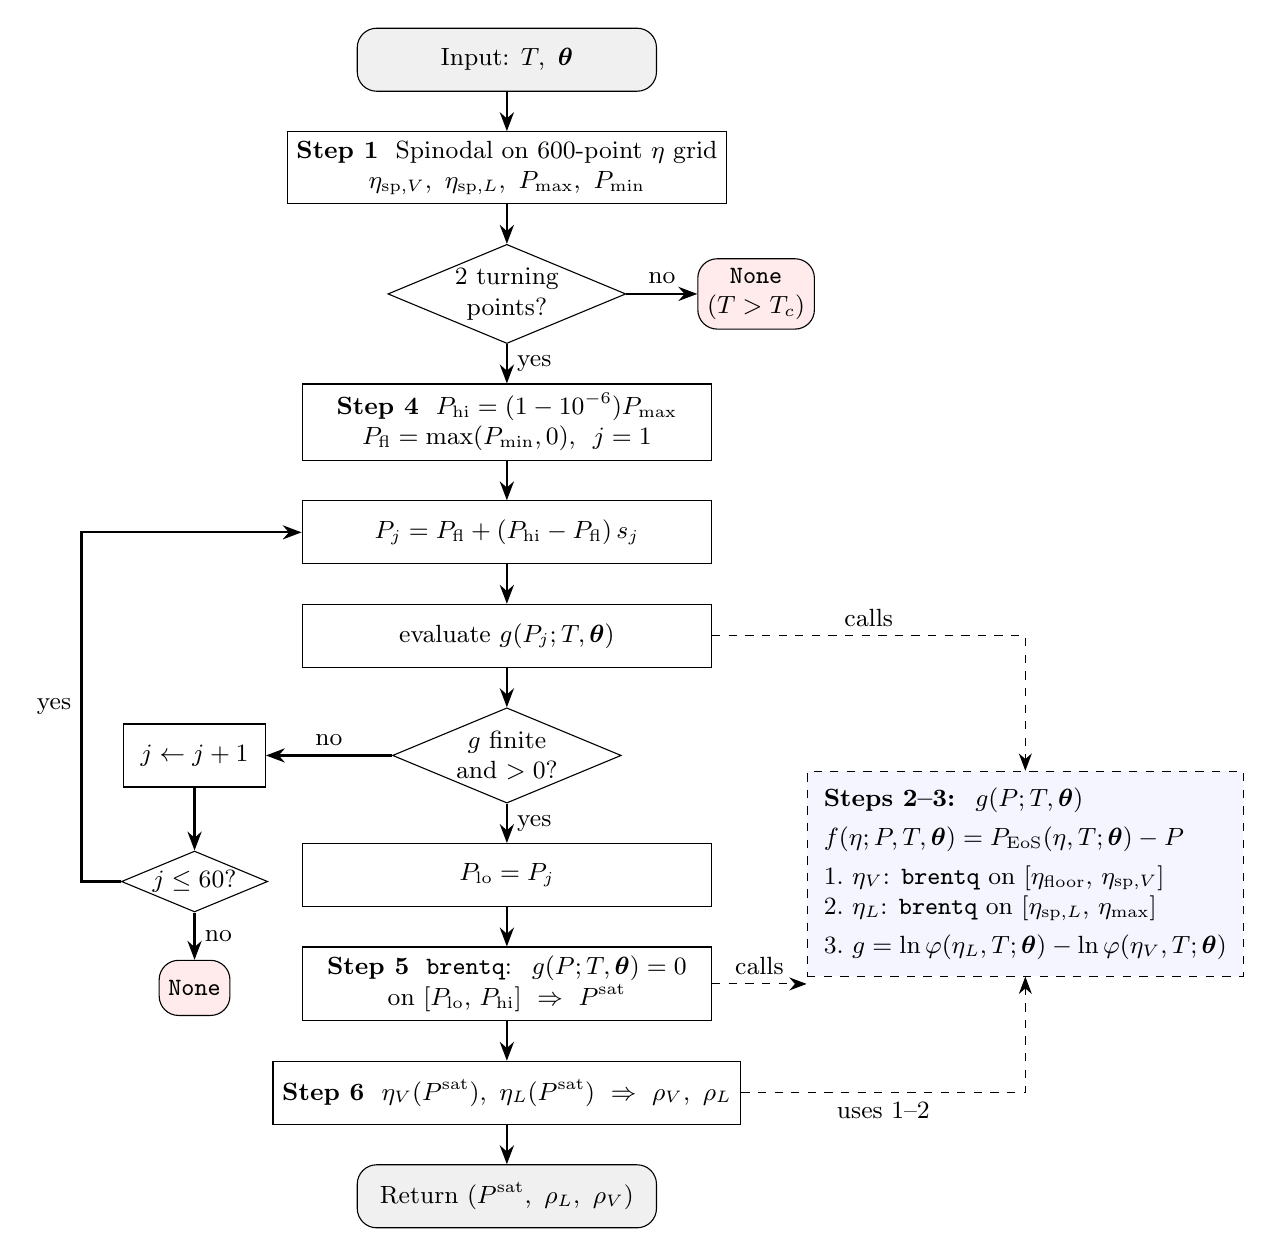
\begin{tikzpicture}[
  font=\small,
  node distance=5mm and 9mm,
  term/.style={rectangle, rounded corners=7pt, draw, fill=gray!12, align=center, minimum width=38mm, minimum height=8mm},
  proc/.style={rectangle, draw, align=center, minimum width=52mm, minimum height=8mm},
  dec/.style={diamond, draw, aspect=2.4, align=center, inner sep=0.5pt},
  none/.style={rectangle, rounded corners=7pt, draw, fill=red!8, align=center, minimum height=7mm},
  sub/.style={rectangle, draw, dashed, align=left, fill=blue!4, inner sep=6pt},
  arr/.style={-{Stealth[length=2.4mm]}, thick},
  call/.style={-{Stealth[length=2.2mm]}, dashed}
]
\node[term] (start) {Input: $T,\ \pth$};
\node[proc, below=of start] (spin) {\textbf{Step 1} \ Spinodal on 600-point $\eta$ grid\\$\etasv,\ \etasl,\ P_{\max},\ P_{\min}$};
\node[dec, below=of spin] (d1) {2 turning\\points?};
\node[none, right=of d1] (n1) {\texttt{None}\\($T>T_c$)};
\node[proc, below=of d1] (win) {\textbf{Step 4} \ $P_{\mathrm{hi}}=(1-10^{-6})P_{\max}$\\$P_{\mathrm{fl}}=\max(P_{\min},0)$, \ $j=1$};
\node[proc, below=of win] (trial) {$P_j = P_{\mathrm{fl}} + (P_{\mathrm{hi}}-P_{\mathrm{fl}})\,s_j$};
\node[proc, below=of trial] (eval) {evaluate $g(P_j;T,\pth)$};
\node[dec, below=of eval] (d2) {$g$ finite\\and $>0$?};
\node[proc, left=16mm of d2, minimum width=18mm] (inc) {$j \leftarrow j+1$};
\node[dec, below=8mm of inc] (d3) {$j\le60$?};
\node[none, below=6mm of d3] (n2) {\texttt{None}};
\node[proc, below=of d2] (lo) {$P_{\mathrm{lo}} = P_j$};
\node[proc, below=of lo] (outer) {\textbf{Step 5} \ \texttt{brentq}: \ $g(P;T,\pth)=0$\\on $[P_{\mathrm{lo}},\,P_{\mathrm{hi}}] \ \Rightarrow\ P^{\mathrm{sat}}$};
\node[proc, below=of outer] (fin) {\textbf{Step 6} \ $\eta_V(P^{\mathrm{sat}}),\ \eta_L(P^{\mathrm{sat}})\ \Rightarrow\ \rho_V,\ \rho_L$};
\node[term, below=of fin] (stop) {Return $(P^{\mathrm{sat}},\ \rho_L,\ \rho_V)$};

\node[sub, right=12mm of outer, yshift=14mm] (g) {%
\textbf{Steps 2--3:} \ $g(P;T,\pth)$\\[3pt]
$f(\eta;P,T,\pth)=\Peos(\eta,T;\pth)-P$\\[3pt]
1.\ $\eta_V$: \texttt{brentq} on $[\eta_{\mathrm{floor}},\,\etasv]$\\
2.\ $\eta_L$: \texttt{brentq} on $[\etasl,\,\eta_{\max}]$\\[3pt]
3.\ $g=\ln\varphi(\eta_L,T;\pth)-\ln\varphi(\eta_V,T;\pth)$};

\draw[arr] (start) -- (spin);
\draw[arr] (spin) -- (d1);
\draw[arr] (d1) -- node[above]{no} (n1);
\draw[arr] (d1) -- node[right]{yes} (win);
\draw[arr] (win) -- (trial);
\draw[arr] (trial) -- (eval);
\draw[arr] (eval) -- (d2);
\draw[arr] (d2) -- node[above]{no} (inc);
\draw[arr] (inc) -- (d3);
\draw[arr] (d3) -- node[right]{no} (n2);
\draw[arr] (d3.west) -- ++(-5mm,0) |- node[pos=0.25,left]{yes} (trial.west);
\draw[arr] (d2) -- node[right]{yes} (lo);
\draw[arr] (lo) -- (outer);
\draw[arr] (outer) -- (fin);
\draw[arr] (fin) -- (stop);
\draw[call] (eval.east) -| node[pos=0.25,above]{calls} (g.north);
\draw[call] (outer.east) -- node[above]{calls} (outer.east -| g.west);
\draw[call] (fin.east) -| node[pos=0.25,below]{uses 1--2} (g.south);
\end{tikzpicture}
\caption{Two nested solvers. The outer \texttt{brentq} moves $P$; every trial $P$ triggers two inner \texttt{brentq} calls on $\eta$. All brackets come from the spinodal.}
\end{figure}

\section{Code map}

\begin{center}
\begin{tabular}{lll}
\toprule
function & computes & step \\
\midrule
\texttt{spinodal(T, comp)} & $\etasv,\ \etasl,\ P_{\max},\ P_{\min}$ & 1 \\
\texttt{\_both\_roots(T, P, comp, eta\_v, eta\_l)} & $\rho\big(\eta_V(P,T;\pth)\big),\ \rho\big(\eta_L(P,T;\pth)\big)$ & 2 \\
\texttt{\_delta\_ln\_phi(P, T, comp, eta\_v, eta\_l)} & $g(P;T,\pth)$ & 3 \\
\texttt{saturation(T, comp)} & $P^{\mathrm{sat}},\ \rho_L,\ \rho_V$ & 4--6 \\
\bottomrule
\end{tabular}
\end{center}

\section{Check: ethane at 250 K}

$\pth = (1.6069,\ 3.5206\ \text{\AA},\ 191.42\ \text{K})$, \ $d(250\ \mathrm{K};\pth) = 3.4781$ \AA.

\begin{center}
\begin{tabular}{ll@{\qquad}ll}
\toprule
\multicolumn{2}{l}{Step 1} & \multicolumn{2}{l}{Steps 4--6} \\
\midrule
$\etasv$ & 0.05403 & $P_{\mathrm{lo}}$ & $2.39\times10^{-6}$ Pa \ ($s_1=10^{-12}$) \\
$\etasl$ & 0.25596 & $P^{\mathrm{sat}}$ & 13.0388 bar \\
$P_{\max}$ & 23.913 bar & $\eta_L$,\ $\eta_V$ & 0.32048, \ 0.016481 \\
$P_{\min}$ & $-92.071$ bar & $\rho_L$,\ $\rho_V$ & 452.03, \ 23.246 kg\,m$^{-3}$ \\
\bottomrule
\end{tabular}
\end{center}

\begin{center}
\begin{tabular}{lcccccc}
\toprule
$P$ / bar & 0.01 & 1 & 10 & 13.0388 & 16 & 20 \\
\midrule
$g(P;\,250\ \mathrm{K},\pth)$ & $+6.958$ & $+2.368$ & $+0.213$ & $\approx 0$ & $-0.151$ & $-0.298$ \\
\bottomrule
\end{tabular}
\end{center}

\section{Limits}

\begin{itemize}
\item The spinodal is a grid point, not the exact turning point, so $P_{\max}$ comes out slightly low and $P_{\min}$ slightly high. Close to $T_c$, where the loop is narrow, this is the first place to look if \texttt{saturation} fails.
\item Each outer iteration costs two inner solves. The cost of one call is roughly one spinodal grid (600 evaluations of $\Peos$) plus a few dozen \texttt{brentq} iterations.
\end{itemize}

\end{document}
